\documentclass[10pt, a4paper, italian]{article}
\usepackage[T1]{fontenc}
\usepackage[utf8]{inputenc}
\usepackage{amsmath, amssymb, amsthm, thmtools, amsfonts, mathtools}
\usepackage{nicefrac}
\usepackage{calc}
\usepackage[pdftex, hyperindex, plainpages=false]{hyperref}
\usepackage[nameinlink]{cleveref} %load before classicthesis (clash)
%\usepackage[nochapters,pdfspacing]{classicthesis}
\usepackage{siunitx}
\usepackage[siunitx]{circuitikz}

\usepackage[a4paper]{geometry}
\usepackage{float}
\usepackage{mdframed}
\usepackage{titling}
\usepackage{booktabs}
\usepackage{graphicx}
\usepackage{caption, subcaption}
\usepackage{xcolor}
\usepackage[italian]{babel}
\usepackage{pgfplots}
\usepackage{listings}
%\usepackage{lmodern}
\usepackage{url}
\usepackage{enumitem}
\usepackage{tikz} %loads after classicthesis (xcolor incompat)

% lets graphicx know path where figures to be included are found
\graphicspath{{../figs/}}
\makeatletter
\def\input@path{{../figs/}}
%or: \def\input@path{{/path/to/folder/}{/path/to/other/folder/}}
\makeatother

% tikz pgf plots setup
\usepgfplotslibrary{external}
\pgfplotsset{compat=1.15}
%\tikzexternalize

% spaces and significant digits/figures for measurements
\sisetup{free-standing-units, space-before-unit, number-unit-product = \;,
scientific-notation = false, round-mode = figures, round-precision = 1,}

% turns all (hyperlinked) references black [default is blue]
\hypersetup{
	linktoc=all,
	colorlinks=true,
	linkcolor=black
}

% code listings config
%\lstset{
%language=Python,
%basicstyle=\ttfamily,
%columns=fullflexible,
%keepspaces=true,
%}

% mdframed (for boxed text) configuration
\mdfsetup{linewidth=0.6pt}

% Default fixed font does not support bold face
\DeclareFixedFont{\ttb}{T1}{txtt}{bx}{n}{12} % for bold
\DeclareFixedFont{\ttm}{T1}{txtt}{m}{n}{12}  % for normal

% Custom colors
\usepackage{color}
\definecolor{deepblue}{rgb}{0,0,0.5}
\definecolor{deepred}{rgb}{0.6,0,0}
\definecolor{deepgreen}{rgb}{0,0.5,0}

% Commands 
\newcommand{\executeiffilenewer}[3]{%
	\ifnum\pdfstrcmp{\pdffilemoddate{#1}}%
		{\pdffilemoddate{#2}}>0%
	{\immediate\write18{#3}}\fi%
}
% input .svg --> .pdf_tex graphs
%\newcommand{\includesvg}[1]{%
%	\executeiffilenewer{#1.svg}{#1.pdf}%
%	{inkscape -z -D --file=#1.svg %
%	--export-pdf=#1.pdf --export-latex}%
%	\input{#1.pdf_tex}%
%}
% Thanks UniPi's Department of Physics E. Fermi
\newcommand{\thanksdf}{(\thanks{Dipartimento di Fisica E.~Fermi,%
Universit\`a di Pisa - Pisa, Italy.}\;)}

% hyperlink to email address
\newcommand{\mail}[1]{\href{mailto:#1}{\textsf{#1}}}

% \vec for bold vectors, instead of overarrows (now "\arrvec")
\let\arrvec=\vec
\renewcommand{\vec}[1]{\boldsymbol #1}
% replaces straight phi with slanted phi
\renewcommand{\phi}{\varphi}
% replaces straight eps with curved epsilon
\newcommand{\eps}{\varepsilon}
% abbreviation for (sub_/super^)scripts of \lim, \sum,... in inline math
\newcommand{\ds}{\displaystyle}

% blackboard/number set letters
\newcommand{\CC}{\mathbb C}
\newcommand{\HH}{\mathbb H}
\newcommand{\KK}{\mathbb K}
\newcommand{\NN}{\mathbb N}
\newcommand{\PP}{\mathbb P}
\newcommand{\QQ}{\mathbb Q}
\newcommand{\RR}{\mathbb R}
\newcommand{\ZZ}{\mathbb Z}

\newcommand{\Abs}[1]{{\left\Vert #1\right\Vert}}
\newcommand{\enclose}[1]{{\left( #1 \right)}}
\newcommand{\Enclose}[1]{{\left[ #1 \right]}}
\newcommand{\floor}[1]{\left\lfloor #1 \right\rfloor}
\newcommand{\ceil}[1]{\left\lceil #1 \right\rceil}
\newcommand{\To}{\rightrightarrows}

% Math operators
\DeclareMathOperator{\divergence}{div}
\renewcommand{\div}{\divergence}
\DeclareMathOperator{\Imaginarypart}{Im}
\renewcommand{\Im}{\Imaginarypart}
\DeclareMathOperator{\Realpart}{Re}
\renewcommand{\Re}{\Realpart}
%\DeclareMathOperator{\arg}{arg}
\DeclareMathOperator{\tg}{tg}
\DeclareMathOperator{\arctg}{arctg}
\DeclareMathOperator{\settsinh}{settsinh}
\DeclareMathOperator{\settcosh}{settcosh}
\DeclareMathOperator{\tr}{tr}
\DeclareMathOperator{\im}{im}
\DeclareMathOperator{\sgn}{sgn}
\DeclareMathOperator{\diag}{diag}

\DeclarePairedDelimiter{\norm}{\lVert}{\rVert}
\DeclarePairedDelimiter{\scalar}{\langle}{\rangle}

% Logarithm with arbitrary base.
% -> log_10
\newcommand{\llog}[1][10]{\log_{#1}}

% Absolute value.
% -> |x|
\newcommand{\abs}[1]{\left| #1 \right|}

% Powers.
% -> x^a
\newcommand{\power}[2][2]{\left( #2 \right)^{#1}}

% Square.
% -> x^2
\newcommand{\sq}[1]{\power[2]{#1}}

% Expansion of the binomial coefficient.
% -> n1!/(n2!(n1 - n2)!)
\newcommand{\binomexpr}[2]{\frac{#1!}{#2!(#1 - #2)!}}

% Expression evaluation at a given point with square brackets.
% -> [x]_{a}
\newcommand{\at}[2]{\left[ #1\right]_{\makebox[-1pt][l]{${\scriptstyle#2}$}}}

% Expression evaluation in an interval.
% -> [x] _{a}^{b}
\newcommand{\eval}[3]{\left.#1%
  \right|_{\makebox[-1pt][l]{${\scriptstyle#2}$}}^{\makebox[-1pt][l]{${\scriptstyle#3}$}}}

% Upright d in math mode (for differentials).
% -> d
\newcommand{\ud}{\mathrm{d}}

% Differential.
% -> dx
\newcommand{\diff}[1][x]{\,\ud{#1}}

% Base command for defining derivatives.
% -> df/dx or d^kf/dx^k
\newcommand{\basederivative}[4][]{%
  \displaystyle%
  \ifx\\#1\\\frac{#4#2}{#4#3}%
  \else%
  \frac{#4^#1#2}{#4#3^#1}%
  \fi%
}

% Total derivative.
% -> df/dx(x) or d^kf/dx^k(x)
\newcommand{\td}[4][]{%
  \basederivative[#1]{#2}{#3}{\ud}%
  \ifx\\#4\\%
  \else%
  \mkern-4mu\left(#4\right)%
  \fi%
}

% Partial derivative.
% -> df/dx(x) or d^kf/dx^k(x)
\newcommand{\pd}[4][]{%
  \basederivative[#1]{#2}{#3}{\partial}%
  \ifx\\#4\\%
  \else%
  \mkern-4mu\left(#4\right)%
  \fi%
}

\newcommand{\intinf}{\int_{-\infty}^{\infty}\!\!\!}

\newcommand{\cinterval}[2]{\left[\, #1,~#2 \,\right]}

\newcommand{\linterval}[2]{\left[\, #1,~#2 \,\right)}

\newcommand{\rinterval}[2]{\left(\, #1,~#2 \,\right]}

\newcommand{\ointerval}[2]{\left(\, #1,~#2 \,\right)}

\newcommand{\prob}[1]{\displaystyle P\left(#1\right)}

\newcommand{\pvalue}{\emph{$p$-value}}

\newcommand{\cond}{\,|\,}

\newcommand{\expect}[1]{\displaystyle E\left[#1\right]}

\newcommand{\mom}[2][]{\displaystyle {\cal M}_{#2}\ifx\\#1\\\else(#1)\fi}

\newcommand{\momalg}[1]{\displaystyle \lambda_{#1}}

\newcommand{\momcen}[1]{\displaystyle \mu_{#1}}

\newcommand{\skewness}{\displaystyle \gamma_1}

\newcommand{\kurtosis}{\displaystyle \gamma_2}

\newcommand{\charf}[1][x]{\phi_{#1}}

\newcommand{\momgenf}[1][x]{M_{#1}}

\newcommand{\fwhm}{{\scriptstyle \textsc{FWHM}}}

\newcommand{\hwhm}{{\scriptstyle \textsc{HWHM}}}

\newcommand{\median}{\mu_{\nicefrac{1}{2}}}

\newcommand{\var}[1]{\ensuremath{\text{Var}\left(#1\right)}}

\newcommand{\cov}[2]{\ensuremath{\text{Cov}\left(#1, #2\right)}}

\newcommand{\corr}[2]{\ensuremath{\text{Corr}\left(#1, #2\right)}}

\newcommand{\like}{\mathcal L}

\newcommand{\likelihood}[2][]{\like\ifx\\#2\\\else(#2\ifx\\#1\\\else;#1\fi)\fi}

\newcommand{\chisq}{\ensuremath{\chi^2}}

\newcommand{\chisquare}[2][]{\chisq\ifx\\#2\\\else(#2\ifx\\#1\\\else;#1\fi)\fi}

\newcommand{\loglikelihood}[2][]{\log\likelihood[#1]{#2}}

\newcommand{\pdf}[3][]{#2(#3\ifx\\#1\\\else;#1\fi)}

\newcommand{\binomialpdf}[2][]{\pdf[#1]{\mathcal B}{#2}}

\newcommand{\multinomialpdf}[2][]{\pdf[#1]{\mathcal M}{#2}}

\newcommand{\poissonpdf}[2][]{\pdf[#1]{\mathcal P}{#2}}

\newcommand{\uniformpdf}[2][]{\pdf[#1]{u}{#2}}

\newcommand{\exponentialpdf}[2][]{\pdf[#1]{\varepsilon}{#2}}

\newcommand{\gausspdf}[2][]{\pdf[#1]{N}{#2}}

\newcommand{\chisquarepdf}[2][]{\pdf[#1]{\wp}{#2}}

\newcommand{\cauchypdf}[2][]{\pdf[#1]{c}{#2}}

\newcommand{\erf}[1]{\ensuremath{\text{erf}\left(#1\right)}}

\newcommand{\dccases}[4][]{#2 \ifx\\#2\\\else=\fi %
  \begin{cases}
    \displaystyle #3 & \text{per variabili discrete}\\
    \displaystyle #4 & \text{per variabili continue}#1
  \end{cases}
}
% sub/super-scriptable for all symbol as math operator 
\newcommand\Scaleforall[1]{\vcenter{\hbox{\scalefont{#1}$\forall$}}}

\DeclareMathOperator*\forevery{%
  \vphantom\sum
  \mathchoice{\Scaleforall{2}}{\Scaleforall{1.4}}{\Scaleforall{1}}{\Scaleforall{0.75}}}
\usepackage{multicol}
\usepackage{diagbox}
\geometry{left=2cm, right=2cm, top=2cm, bottom=2cm}

% indexes subsections with letters, sections with numbers (1.a, 1.b, ...)
\renewcommand{\thesubsection}{\thesection.\alph{subsection}}

% lets graphicx know path where figures to be included are found
\graphicspath{{../figs/}}

\author{Gruppo 1.AC \\ Matteo Rossi, Bernardo Tomelleri}
\title{EsD2: Costruzione di D-Latch, contatori e shift-register}
\begin{document}
\date{\today}
\maketitle

\section*{Misura componenti dei circuiti}
\begin{table}[htbp]
\centering
\begin{tabular}{ccc}
\toprule
Resistenze $[\si{\ohm}]$ & $R$ & $\sigma R$ \\
\midrule
\midrule
$R\ped{pot1}$	& 9.53 k	& 0.08 k 		\\
$R\ped{pot2}$	& 9.78 k	& 0.08 k 		\\

\bottomrule     
\end{tabular}
\caption{Valori di resistenza misurati per i componenti passivi dei circuiti
studiati. \label{tab: rmesM}}
\end{table}

Riportiamo per completezza anche il valore della tensione continua di
alimentazione per i circuiti integrati misurata con il multimetro
\begin{align*}
V_{CC} &= 4.99 \pm 0.03 \si{\V} \\
\end{align*}

\subsection*{Nota sul metodo di fit}
Per determinare i parametri ottimali e le rispettive covarianze si \`e
implementato in \verb+Python+ un algoritmo di fit basato sui minimi quadrati
mediante la funzione \emph{curve\_fit} della libreria \texttt{SciPy}.

\setcounter{section}{0}
%=======================
\section{D-Latch con Enable}
\begin{minipage}{0.7\textwidth}
Si vuole studiare il funzionamento di un D-Latch con bit di Enable costruito utilizzando solo porte NAND appartenenti all'integrato SN74LS00, utilizzando come riferimento lo schema in \cref{fig: schem_dlatch}.
Il circuito si ottiene a partire da un SR-Latch con Enable costruito tramite l'uso di porte NAND, andando poi a inviare all'ingresso R il segnale negato di S; la porta S sarà quindi rinominata in D.
\end{minipage}
\begin{minipage}{0.3\textwidth}
	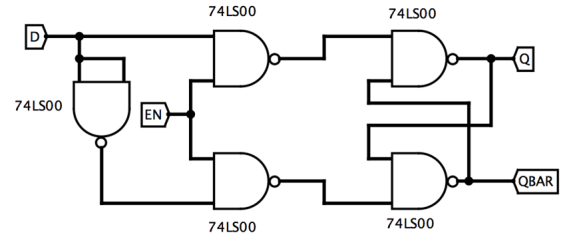
\includegraphics[width=\textwidth]{Schem_DLATCH}
	\captionof{figure}{\label{fig: schem_dlatch}}
\end{minipage}
\subsection{Descrizione del funzionamento}
Partendo da un SR-Latch, inviamo all'ingresso R il segnale negato di S: in questo modo i due bit non avranno mai lo stesso valore, andando così a prevenire lo stato proibito tipico del Latch e diminuendo effettivamente il numero di ingressi al circuito.
Il nuovo circuito avrà quindi solo due ingressi, uno di enable che mi permette di sovrascrivere il segnale in uscita dal Latch e l'altro di Dato; sarà quindi chiamato D-Latch.
Si può quindi costruire una tabella di verità per i D-Latch a partire da quella dei Latch SR.

\begin{table}[htbp]
\centering
\begin{tabular}{cc|cc}
\toprule
$E$ & $D$ & $Q'$ & $\overline{Q'}$ \\
\midrule
\midrule
0&0&Q&$\overline{Q}$\\
0&1&Q&$\overline{Q}$\\
1&0&0&1\\
1&1&1&0\\
\bottomrule
\end{tabular}
\caption{Tabella di verità del circuito D-Latch
\label{tab: D-Latch}}
\end{table}

Finché il bit di enable è 0, si mantiene lo stato di Hold, e in uscita da Q avrò sempre lo stesso valore.
Quando invece il bit di enable vale 1, l'uscita Q assume il valore di D.
Il circuito ha quindi il compito di memorizzare un bit: mentre E è 1 viene memorizzato un valore all'interno del Latch tramite D; quando poi E torna a essere 0 il circuito "ricorderà" il valore di D nell'istante immediatamente precedente al cambiamento di E.
\subsection{Verifica del funzionamento}
Vogliamo ora verificarne il funzionamento; dopo aver montato il circuito utilizziamo la funzione Pattern per inviare due segnali di clock della stessa frequenza sfasati di $\pi /2$ a D e E.
Utilizziamo poi Logic per acquisire i valori di D,E e Q,$\overline{Q}$ in funzione del tempo.
\begin{figure}
	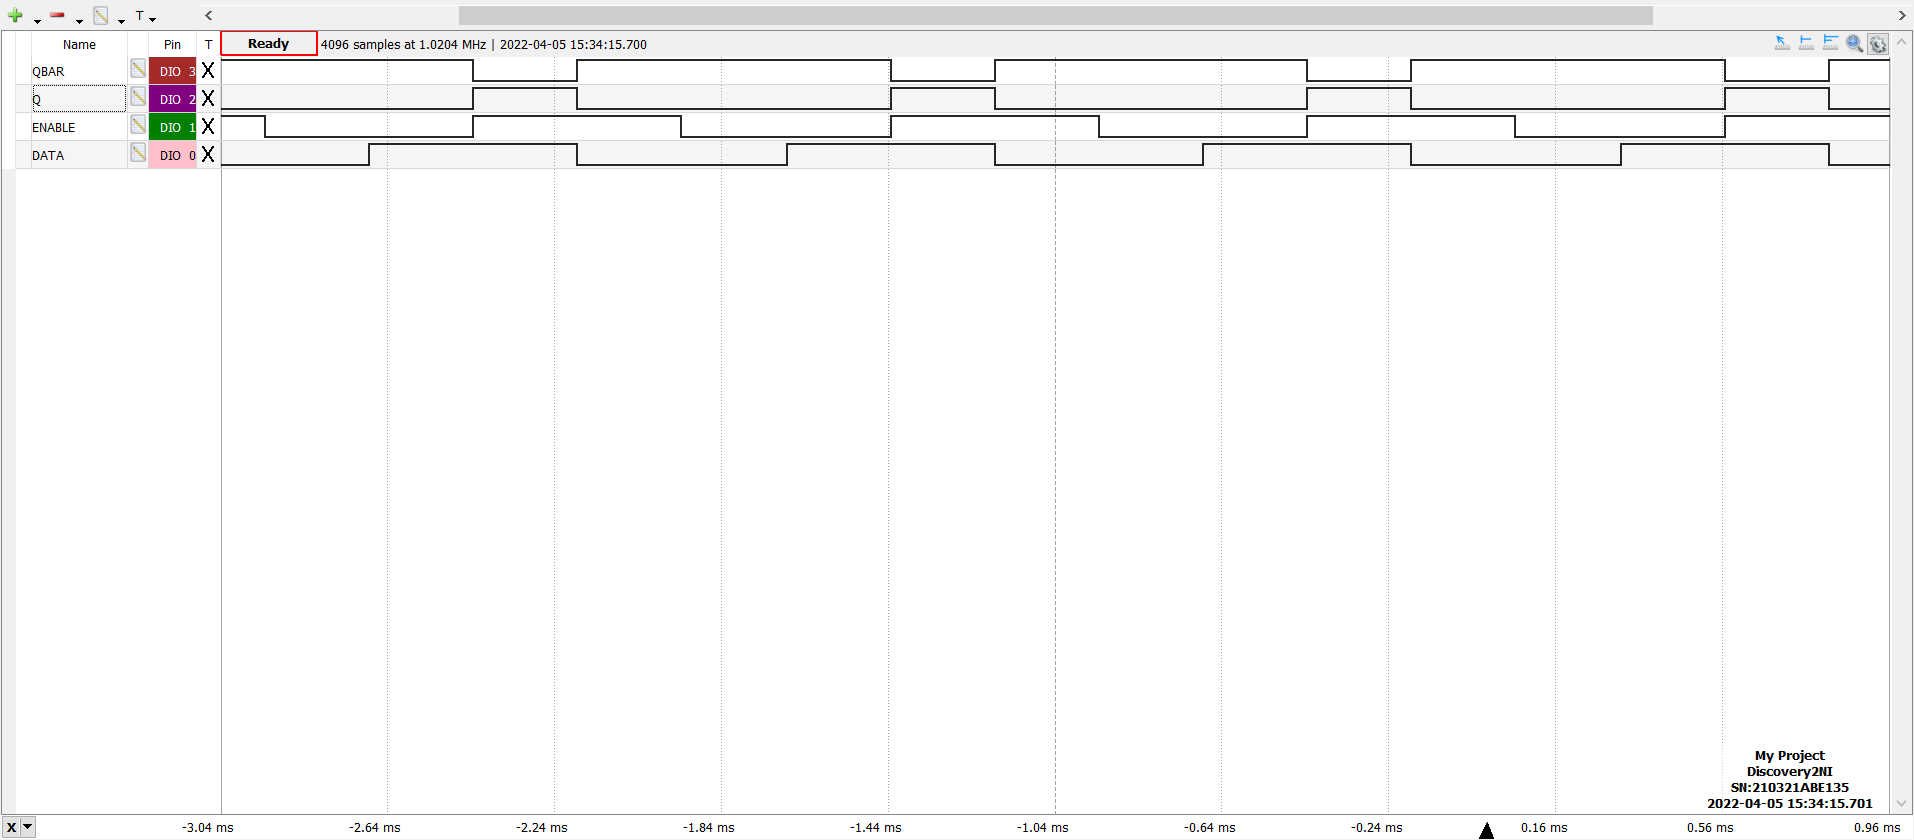
\includegraphics[width=\textwidth]{latch1}
	\label{fig: Log_DLATCH1}
	\caption{Acquisizione temporale con Logic dei segnali in entrata e in uscita da un D-Latch; tra i due segnali D ed E c'è uno sfasamento di $90 \degree$}
\end{figure}
\begin{figure}
	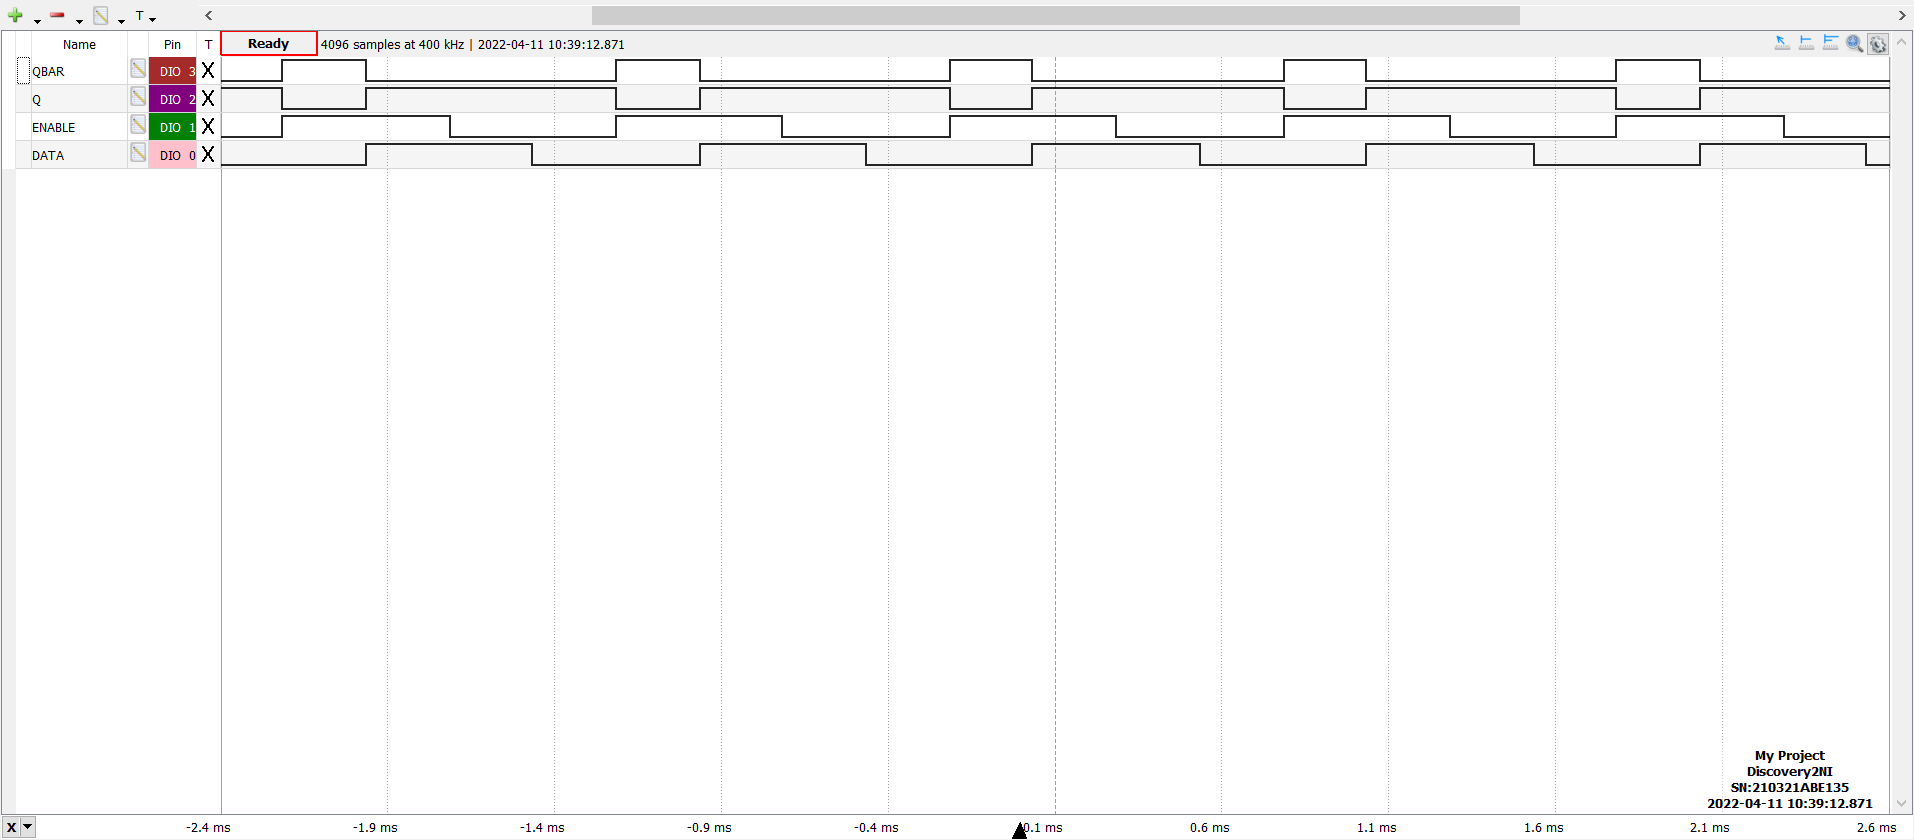
\includegraphics[width=\textwidth]{latch2}
	\label{fig: Log_DLATCH2}
	\caption{Acquisizione temporale con Logic dei segnali in entrata e in uscita da un D-Latch; tra i due segnali D ed E c'è uno sfasamento di $-90 \degree$}
\end{figure}
Dalle \cref{fig: Log_DLATCH1} e \cref{fig: Log_DLATCH2} possiamo notare che i valori di Q e $\overline{Q}$ sono sempre uno il negato dell'altro, il valore di Q equivale a D nel caso in cui E=1, e che il valore di Q viene salvato quando E scende a 0; inoltre mentre E=0 il valore di D non va ad influire sul valore di Q.
Da questo possiamo dedurre che il circuito ha il comportamento atteso.
\subsection{Ritardi dell'uscita Q}
%TODO AMOGUS AAAAAAAAAAAAAAAAAAAAAAAAAAAAAAAAAAAAAAAAAAAAAAA

%=======================

\section{Shift Register con edge-triggered D-Flip Flop}
\begin{minipage}{0.6\textwidth}
Si vuole ora costruire uno Shift Register a 4 bit a partire dagli integrati della serie SN74LS74, secondo lo schema in \cref{fig: schem_shift} e verificarne il funzionamento.
\end{minipage}
\begin{minipage}{0.4\textwidth}
	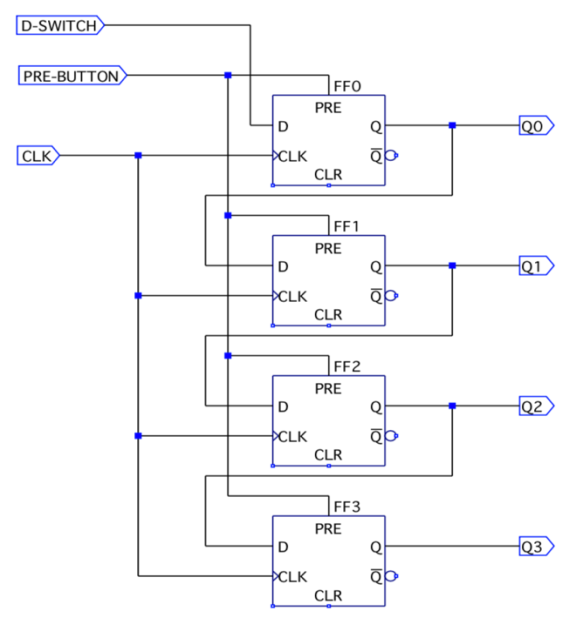
\includegraphics[width=\textwidth]{schem_shift}
	\captionof{figure}{\label{fig: schem_shift}}
\end{minipage}
\subsection{Funzionamento tramite Preset}
Per prima cosa dopo aver montato il circuito verifichiamo la sincronicità delle commutazioni delle uscite.
Dopo aver controllato che le uscite Q0, Q1, Q2 e Q4 fossero nello stato 0000, mantenendo il segnale di clock e il D-Switch scollegati abbiamo utilizzato la funzione StaticIO di wavegen per pilotare il pin PRE-BUTTON di \cref{fig: schem_shift} tramite un button di tipo pressed=0 e released=1 e  Logic per programmare un trigger che facesse partire l'acquisizione alla pressione del button, osservando le tracce prodotte dai 4 segnali in uscita.
\begin{figure}
	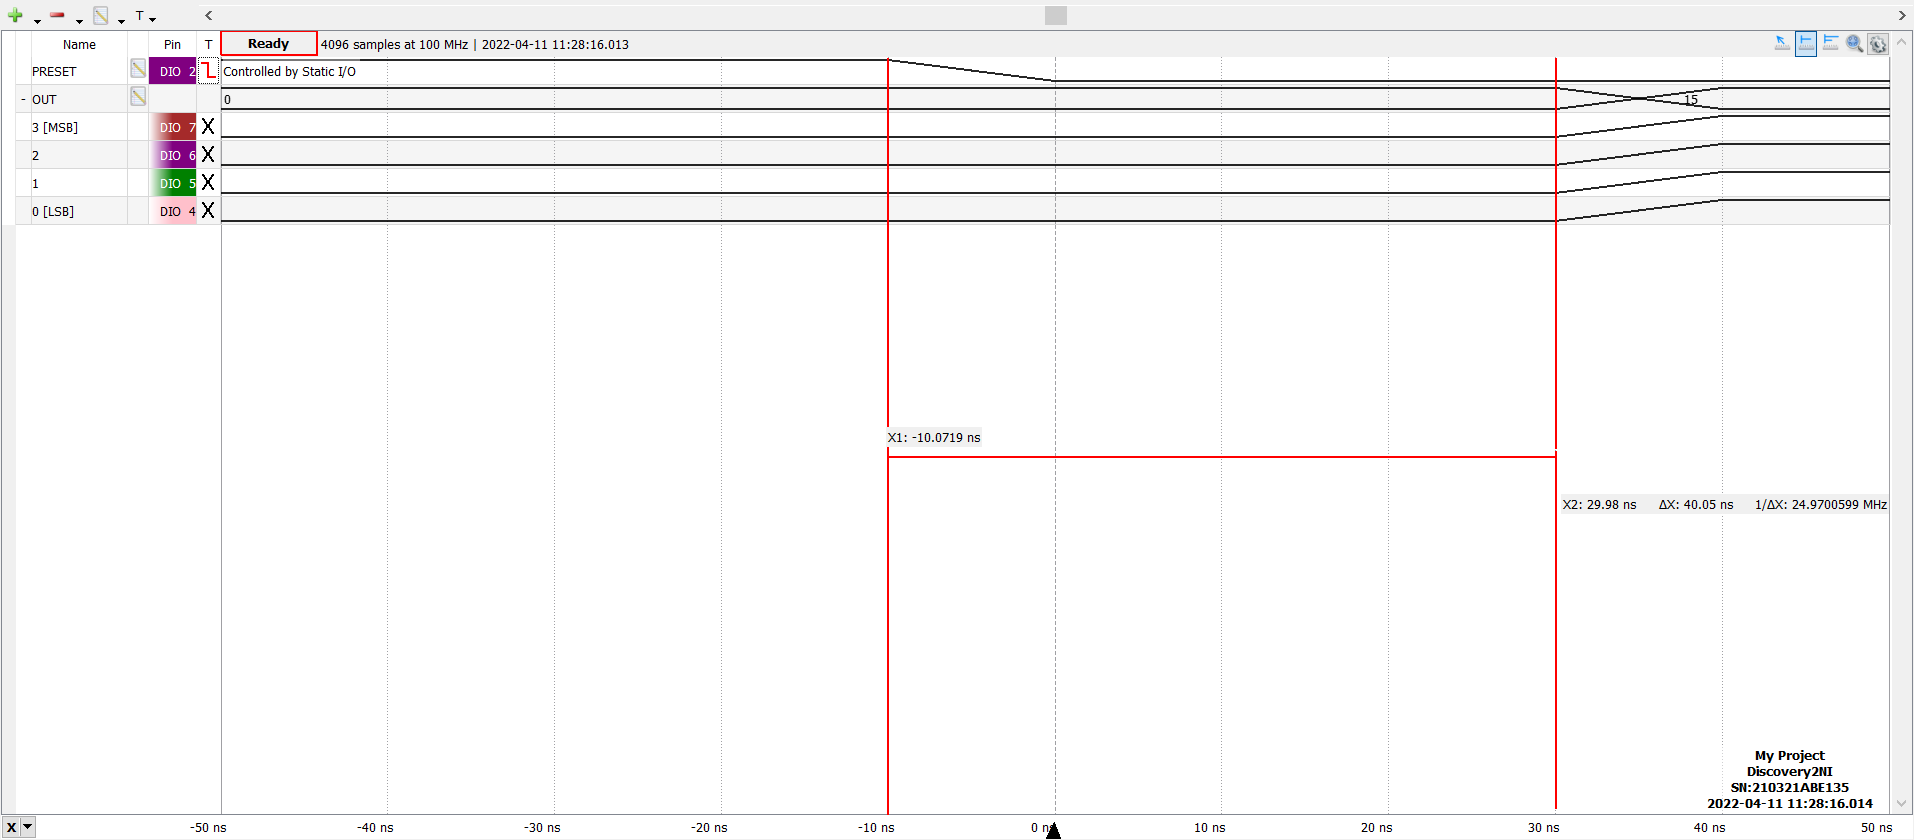
\includegraphics[width=\textwidth]{3.trans}
	\label{fig: Shift_reg_trans}
	\caption{Acquisizione temporale con Logic dei segnali di PRE-BUTTON e i 4 segnali in uscita da un registro a scorrimento di 4 bit come illustrato in \cref{fig: schem_shift}}
\end{figure}
Dalla figura \cref{fig: Shift_reg_trans} vediamo che le commutazioni delle uscite avvengono in maniera sincrona, a un $\Delta T = 40 \si{n\s}$ a partire dalla pressione del pulsante di preset; successivamente le 4 uscite hanno raggiunto lo stato 1111.
\subsection{Funzionamento tramite Clock}
\label{Clock_reg}
A questo punto si vuole verificare il funzionamento del registro a scorrimento tramite un segnale di clock.
Possiamo quindi costruire una tabella di verità in funzione del tempo del registro a partire dal periodo $T$ del clock inviato:
\begin{table}[htbp]
\centering
\begin{tabular}{c|cc}
\toprule
$t=t'$ & $t=t' + \Delta T$ & $ $\\
\midrule
\midrule
$Q_0$&$Q_0'$&$Q_0'$\\
$Q_1$&$Q_0$(t=t')&$Q_0$(t=t')\\
$Q_2$&$Q_1$(t=t')&$Q_0$(t=t'-$\Delta T$)\\
$Q_3$&$Q_2$(t=t')&$Q_0$(t=t'-2$\Delta T$)\\
\bottomrule
\end{tabular}
\caption{Tabella "di verità" di un registro a scorrimento, $Q_0'$ è il valore che viene inviato durante l'impulso di clock tramite il D-SWITCH
\label{tab: S-register}}
\end{table}
Come strategia per la verifica, utilizzeremo inizialmente il pulsante di preset per inizializzare tutte le uscite a 1, successivamente imposteremo il D-Switch tramite StaticIO come switch di tipo Push-Pull impostandolo a 0
e invieremo un segnale di clock dell'ordine di 1 Hz. Utilizzeremo quindi Logic per acquisire gli andamenti nel tempo delle uscite.
Dunque ci si aspetta che dopo 3 periodi di clock (3 secondi) a partire da quando l'uscita Q0 diventa 0, tutte le uscite diventino 0, e che aspettando ulteriormente questi valori non cambino.
\begin{figure}
	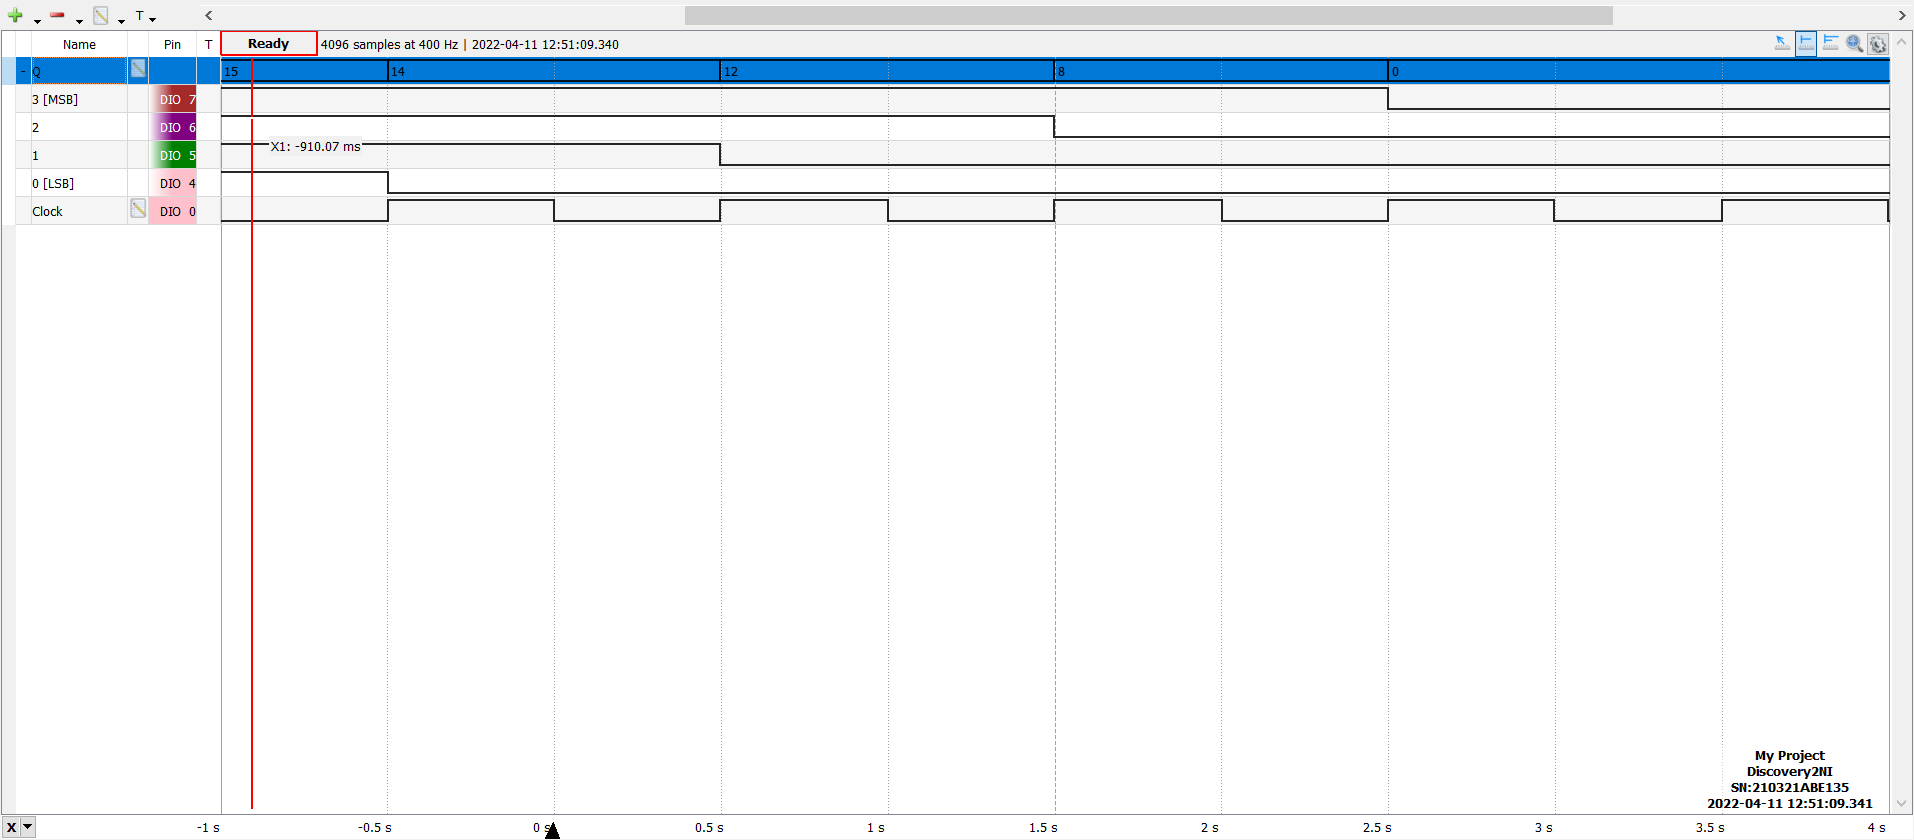
\includegraphics[width=\textwidth]{3.c}
	\label{fig: Shift_reg_clock}
	\caption{Acquisizione temporale con Logic dei segnali in uscita da un registro a scorrimento di 4 bit come spiegato in \cref{Clock_reg}}
\end{figure}
Dalla \cref{fig: Shift_reg_clock} si verifica quanto detto prima, e le 4 uscite diventano (e si mantengono nel tempo visto che il D-Switch resta fisso a 0) tutte quante 0.
Da questo si intuisce che collegando l'uscita $Q_3$ all'entrata del D-switch, possiamo generare una sequenza periodica.
Dopo aver impostato tutte le uscita a 0, si collega l'uscita $\overline{Q_3}$ all'entrata D del primo Flip-Flop e si  invia un clock di frequenza pari a 1 kHz al circuito.
Ci si aspetta che, prendendo un'uscita a caso, si osservi un segnale di clock di frequenza un quarto di quella di clock: questo effetto è dovuto a come la sequenza viene caricata nel registro a partire dall'uscita $\overline{Q_3}$.
In generale supponendo che nel circuito ci siano in cascata n Flip-Flop, e che tutte le uscite siano inizializzate a 0, in una qualsiasi delle uscite otterrò un clock di frequenza pari a $\frac{f_{clock}}{n}$.
\begin{figure}
	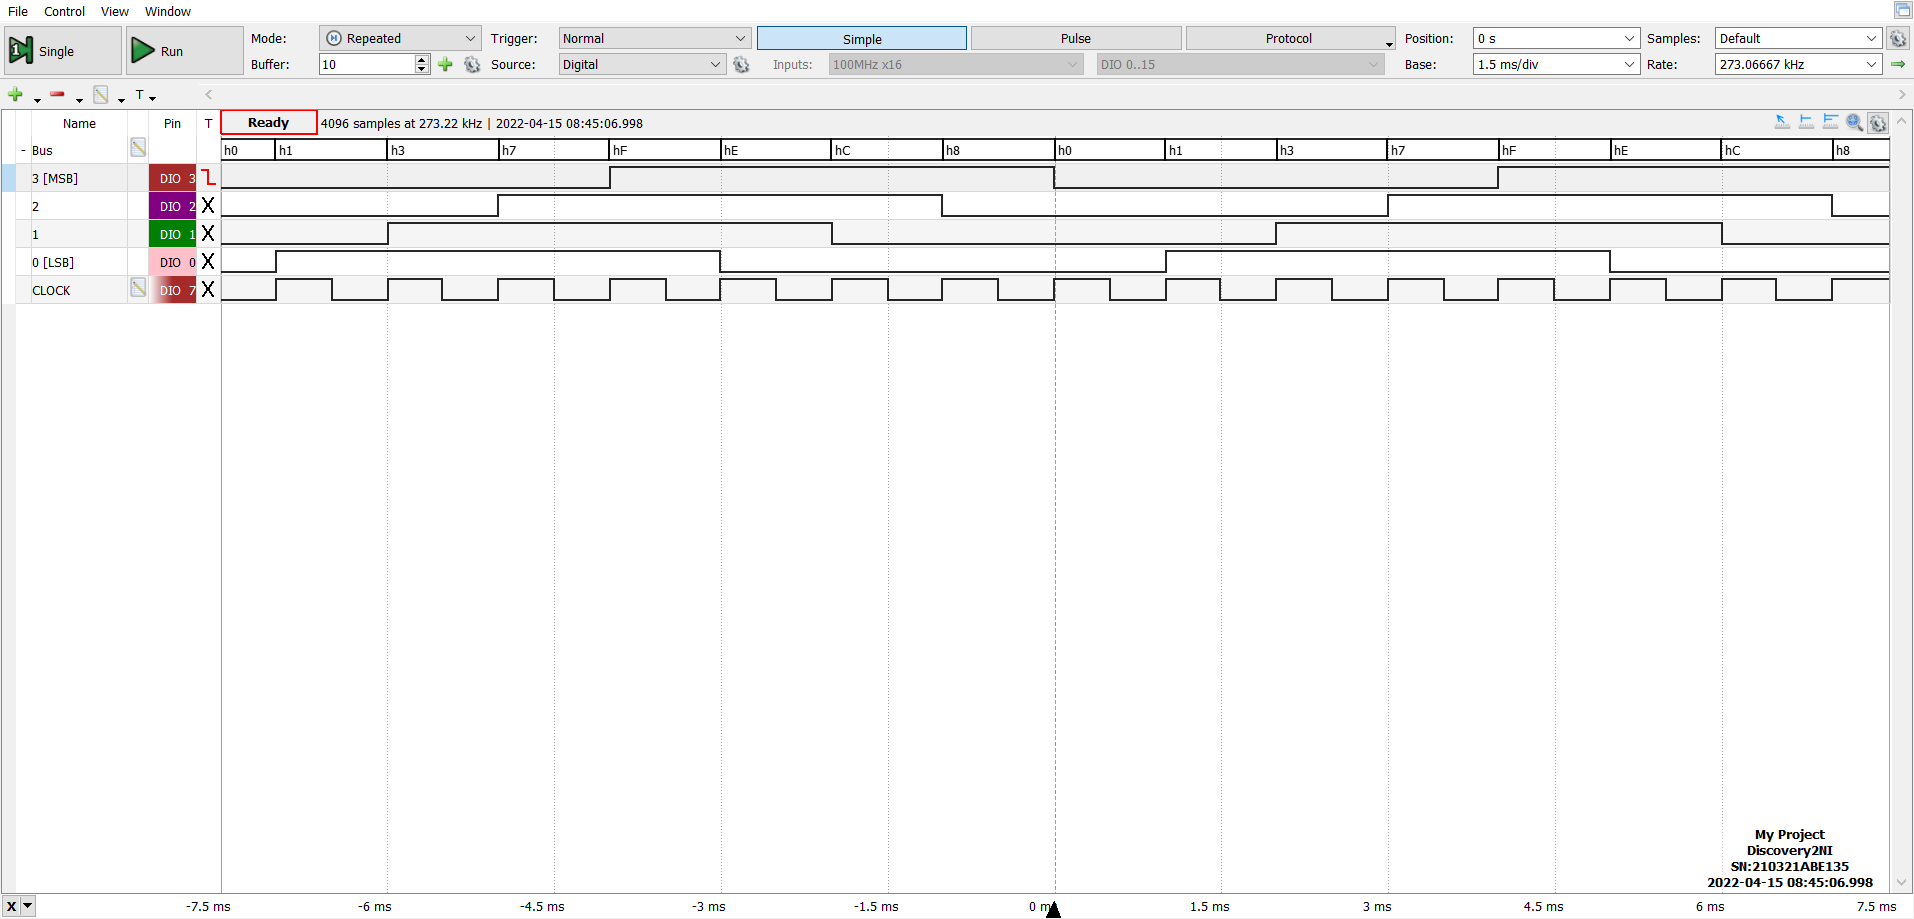
\includegraphics[width=\textwidth]{3.e}
	\label{fig: Shift_reg_seq}
	\caption{Acquisizione temporale con Logic dei segnali in uscita da un registro a scorrimento di 4 bit con l'ultima uscita negata collegata all'entrata del primo flip flop}
\end{figure}
%=======================
\section{Generatore di sequenze pseudo casuali}
\begin{minipage}{0.6\textwidth}
Si vuole ora costruire un generatore di sequenze pseudo-casuali a 4 bit utilizzando lo shift register costruito in precedenza e una porta XOR; la schematica del circuito che utilizzeremo è riportato in figura \cref{fig: schem_gen}.
\end{minipage}
\begin{minipage}{0.4\textwidth}
	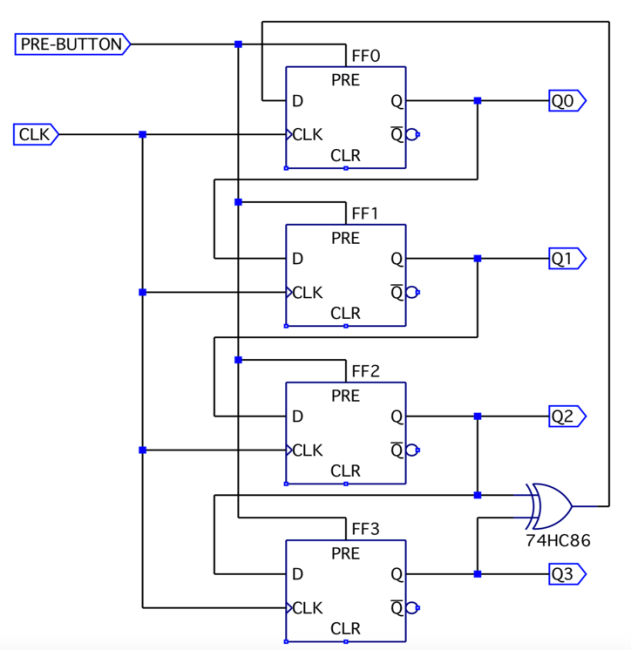
\includegraphics[width=\textwidth]{schem_gen}
	\captionof{figure}{\label{fig: schem_gen}}
\end{minipage}
\subsection{Funzionamento e scelta dei TAP}
Dopo aver montato il circuito si inizializzano tutti Flip-Flop a 1 e si invia un segnale di clock a 10 kHz per verificare il funzionamento: 
essendo il registro di lunghezza pari a 4 bit, dalla teoria ci aspettiamo che la sequenza si ripeta dopo $2^4 = 16$ eventi al massimo, condizione che si ottiene utilizzando come TAP (segnali in ingresso alla porta XOR, la cui uscita sarà inviata all'entrata D del primo Flip-Flop) le uscite $Q_2$ e $Q_3$. 

\begin{figure}
	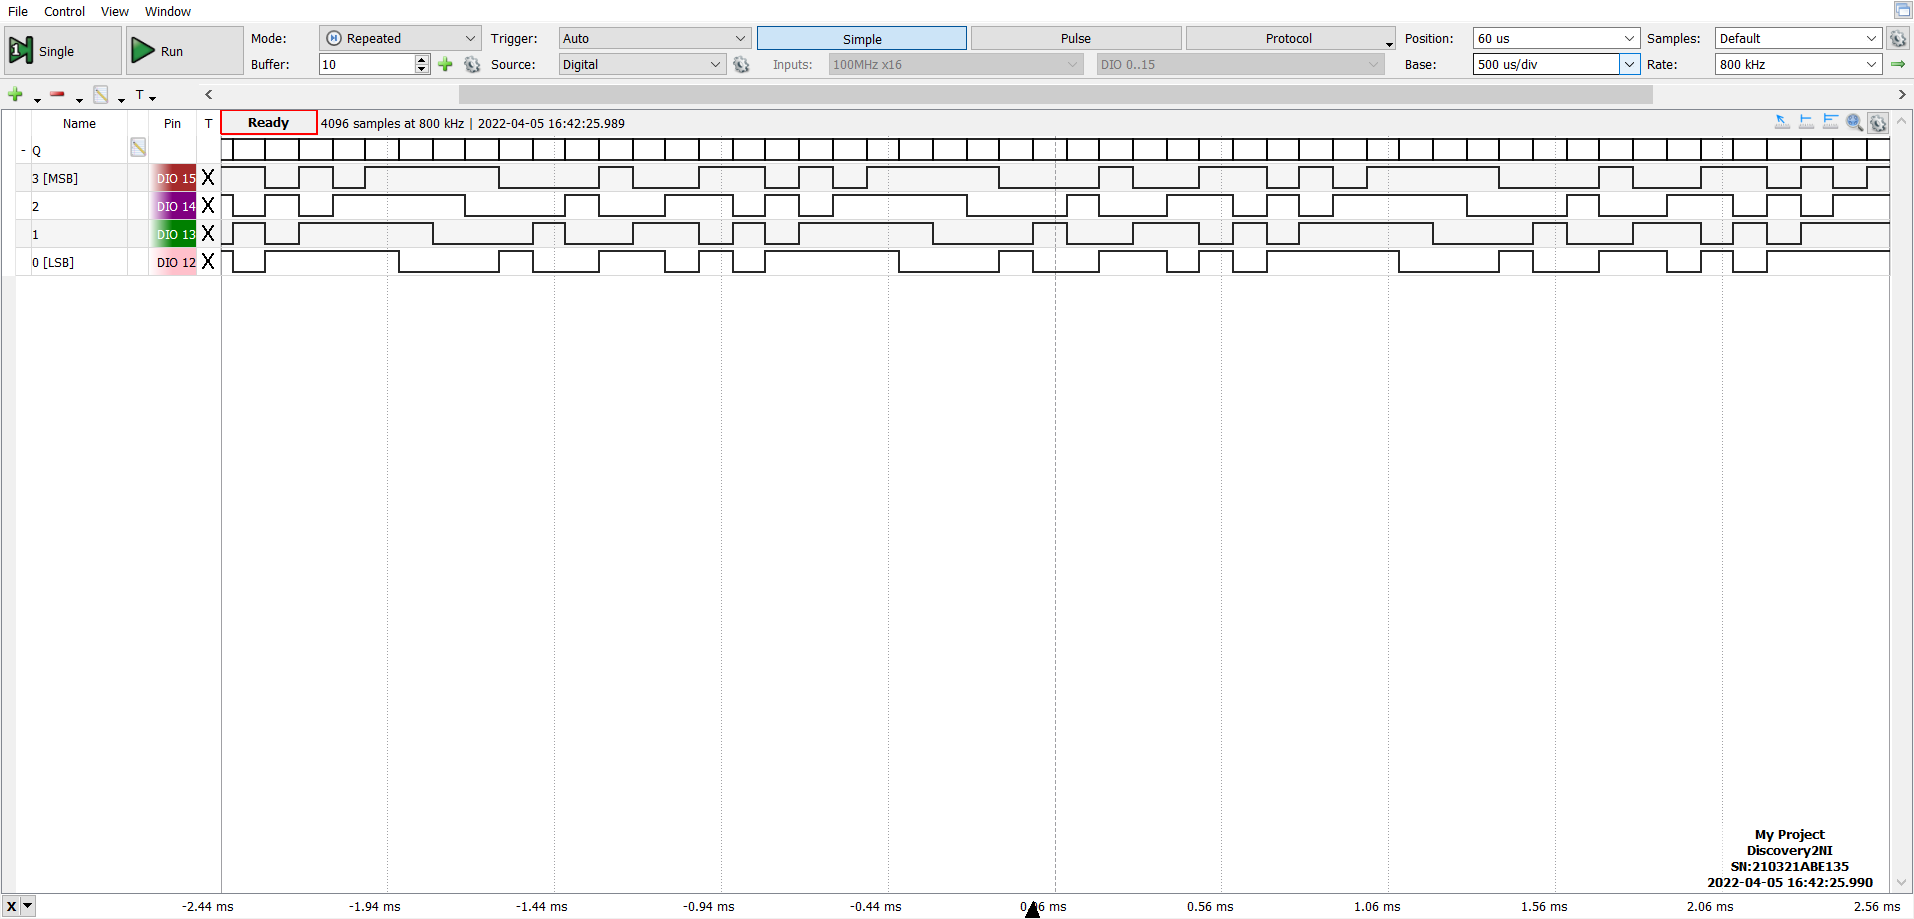
\includegraphics[width=\textwidth]{4.b}
	\caption{\label{fig: TAP_23}Acquisizione temporale con Logic del bus in uscita dal generatore di sequenze psudo-casuale descritto in \cref{fig: schem_gen}}
\end{figure}

Dalla \cref{fig: TAP_23} si verificano le aspettative per cui la sequenza generata a una qualsiasi uscita si ripete ogni 16 periodi di clock (essendo uno shift register la sequenza nelle altre uscite sarà la medesima, solo che saranno sfasate lungo l'asse temporale le une con le altre).
Si provano quindi altre combinazioni di TAP, per verificare che la scelta di utilizzare l'uscita $Q_2$ e $Q_3$ produce una sequenza più lunga rispetto a qualunque altra configurazione
\begin{figure}
	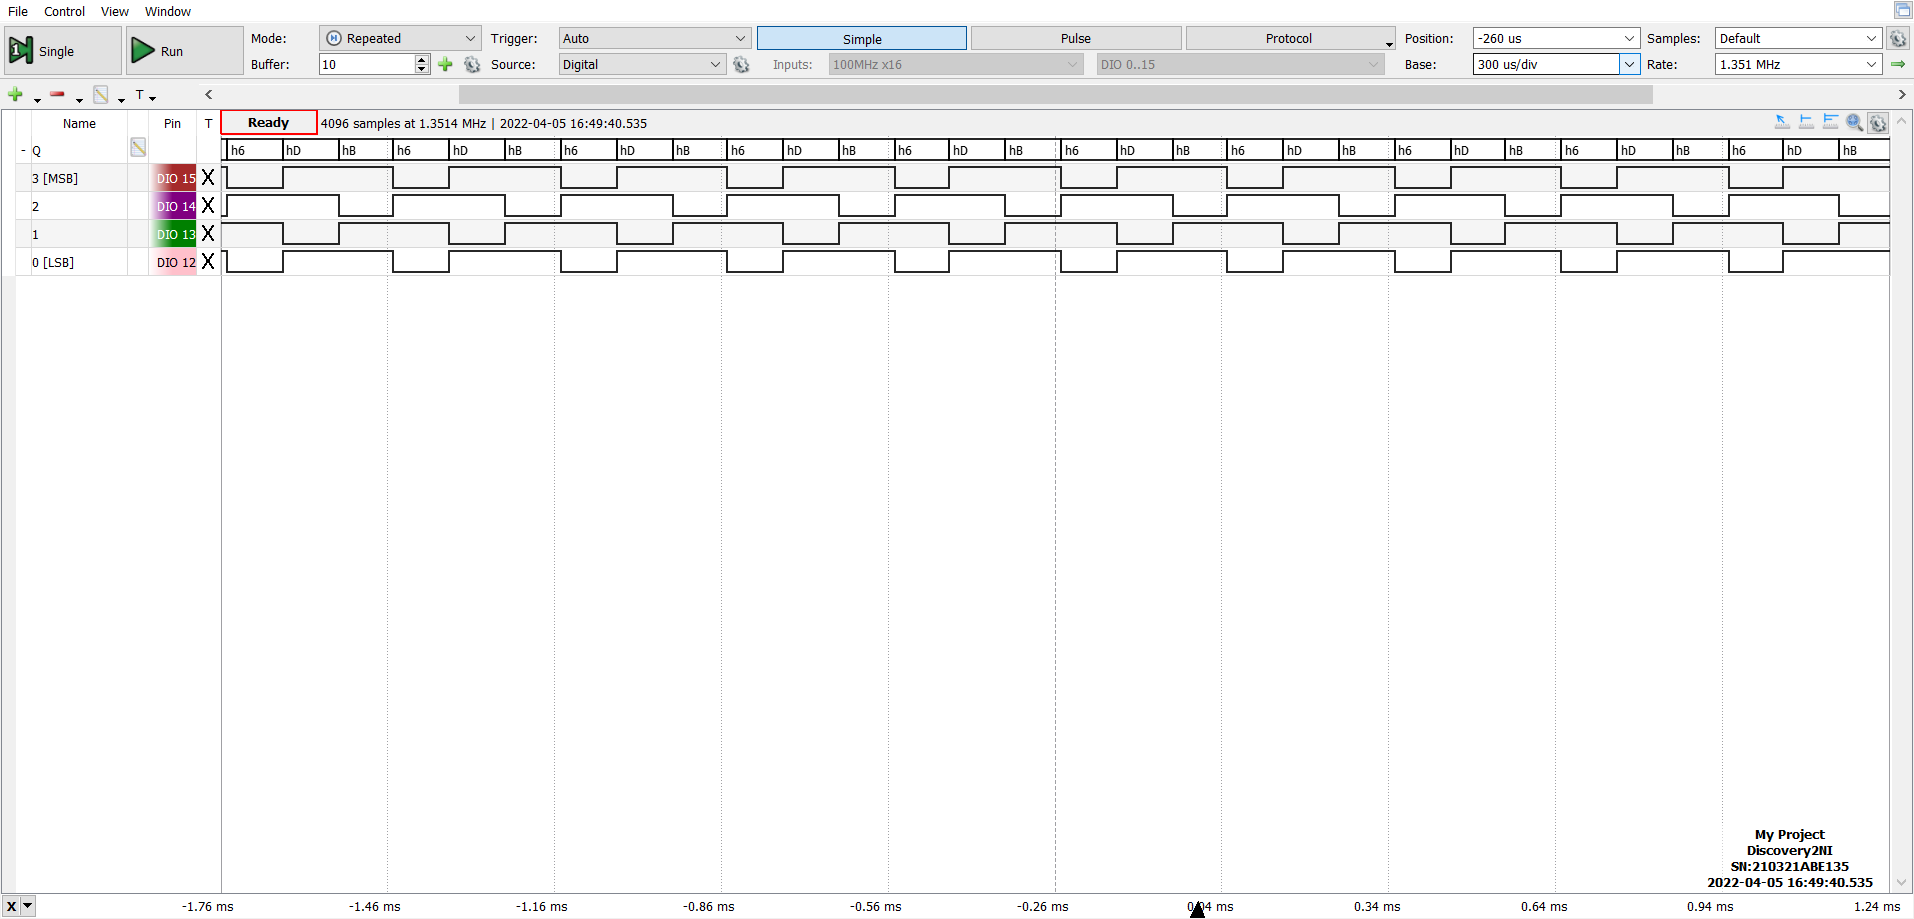
\includegraphics[width=\textwidth]{4.b_10}
	\label{fig: TAP_10}
	\caption{Acquisizione temporale con Logic del bus in uscita dal generatore di sequenze psudo-casuale con TAP sulle uscite $Q_0$ e $Q_1$, la sequenza si ripete ogni 4 eventi}
\end{figure}
\begin{figure}
	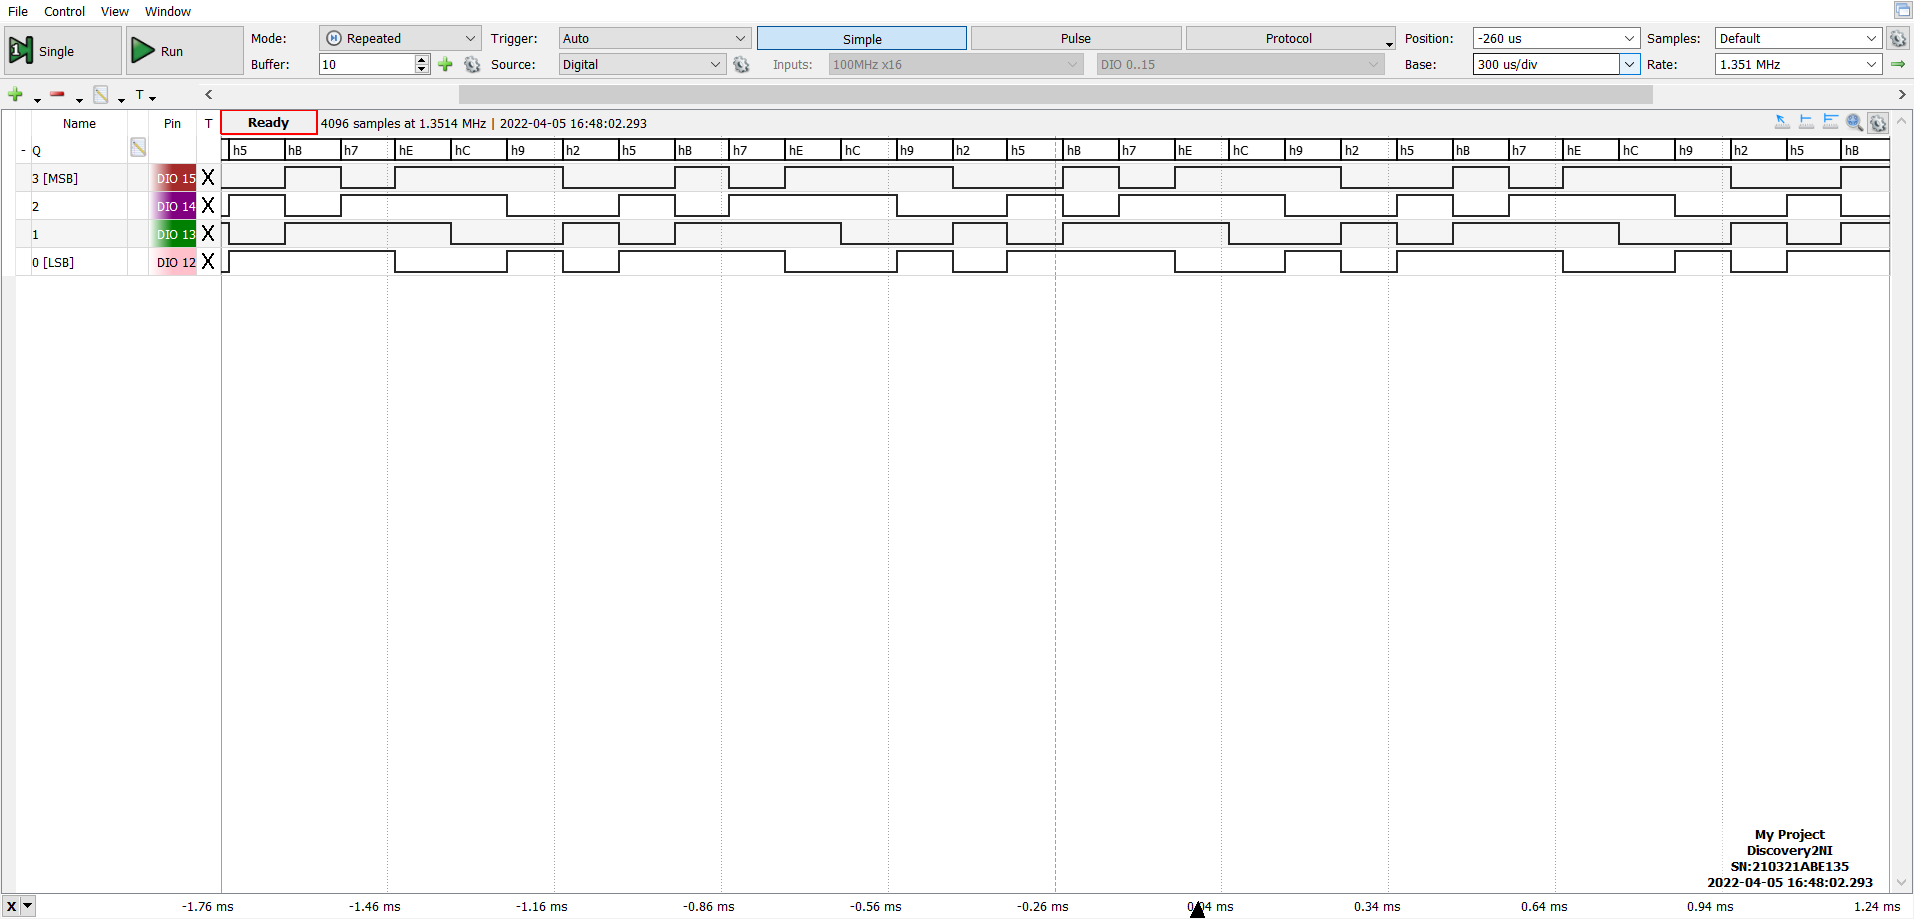
\includegraphics[width=\textwidth]{4.b_21}
	\label{fig: TAP_21}
	\caption{Acquisizione temporale con Logic del bus in uscita dal generatore di sequenze psudo-casuale con TAP sulle uscite $Q_2$ e $Q_1$, la sequenza si ripete ogni 8 eventi}
\end{figure}
\begin{figure}
	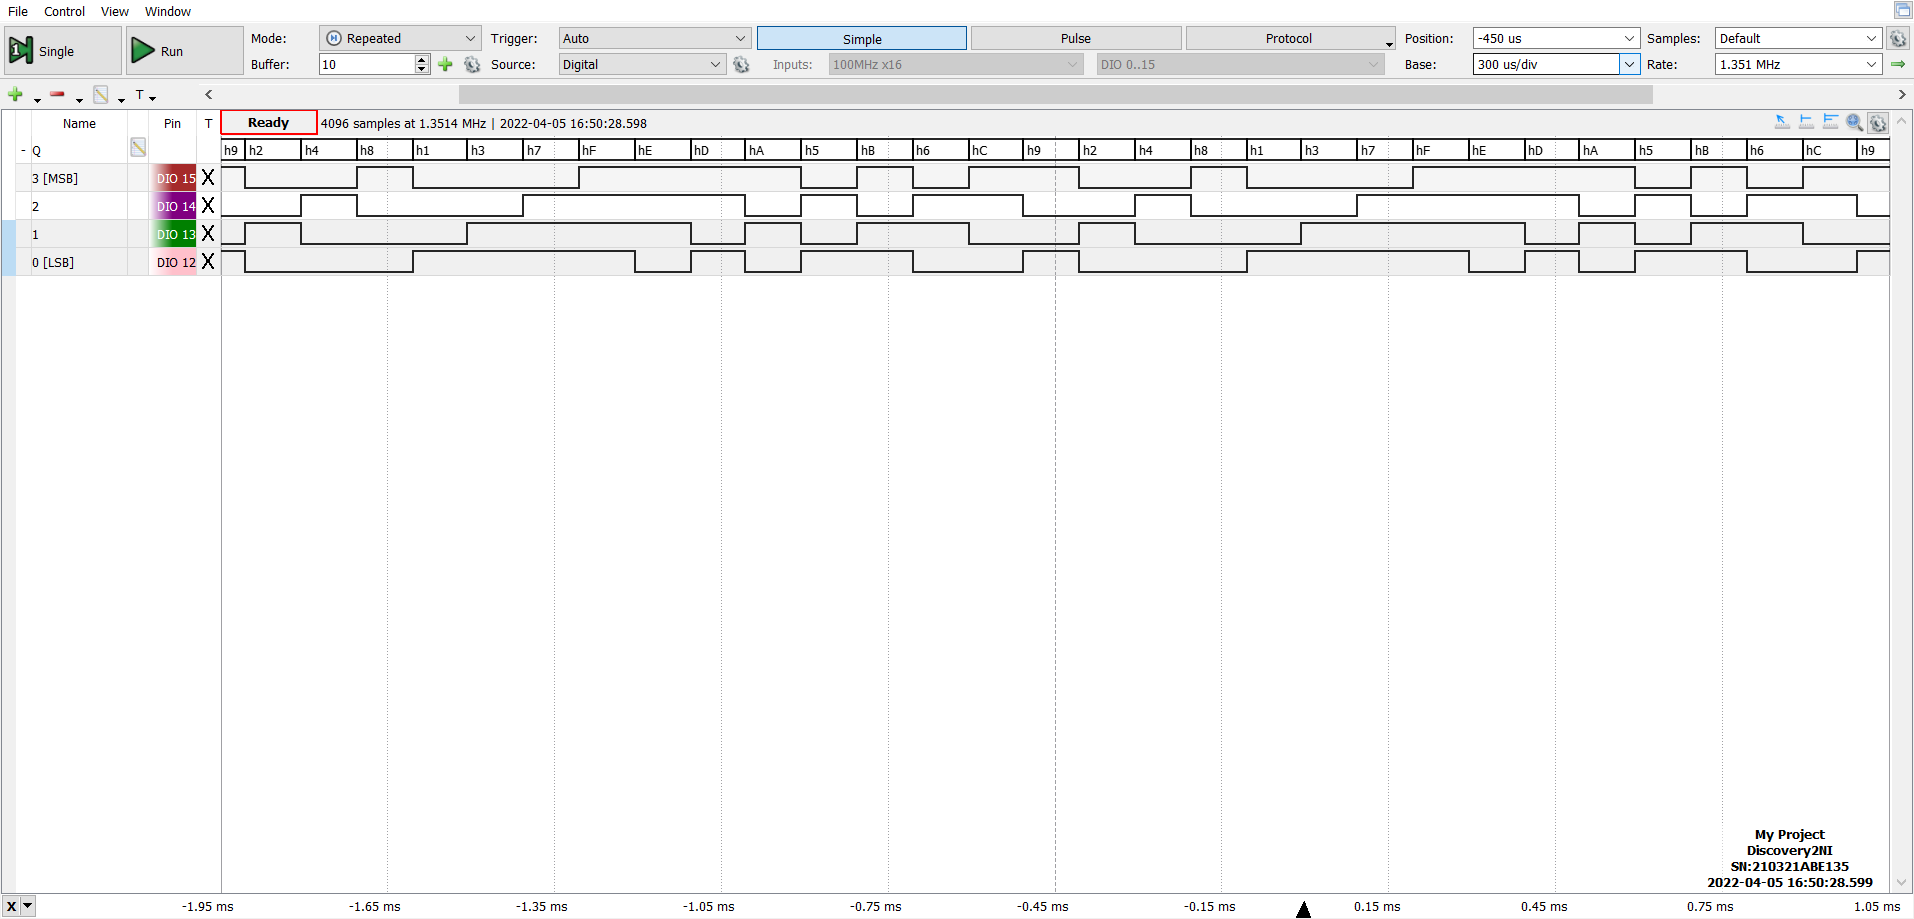
\includegraphics[width=\textwidth]{4.b_30}
	\label{fig: TAP_30}
	\caption{Acquisizione temporale con Logic del bus in uscita dal generatore di sequenze psudo-casuale con TAP sulle uscite $Q_0$ e $Q_3$, la sequenza si ripete ogni 16 eventi}
\end{figure}
%=======================
\section{Divisore di frequenza}
\begin{minipage}{0.6\textwidth}
Si vuole infine costruire un divisore di frequenza a partire da un contatore binario a 4 bit, utilizzando l'integrato SN74LS163, presente in \cref{fig: schem_counter}. Si vuole innanzitutto verificarne il funzionamento. 
\end{minipage}
\begin{minipage}{0.4\textwidth}
	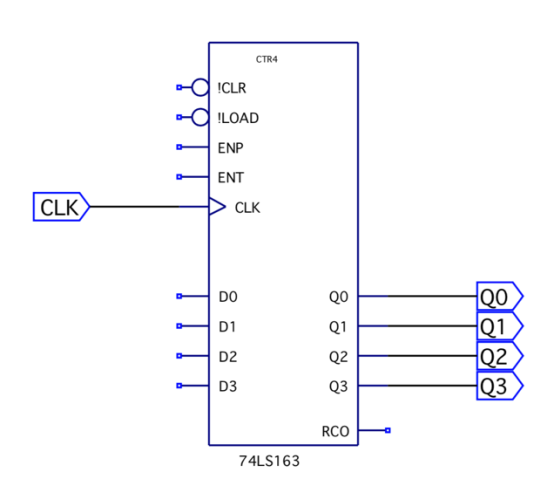
\includegraphics[width=\textwidth]{schem_con}
	\captionof{figure}{\label{fig: schem_counter}}
\end{minipage}


\begin{figure}
	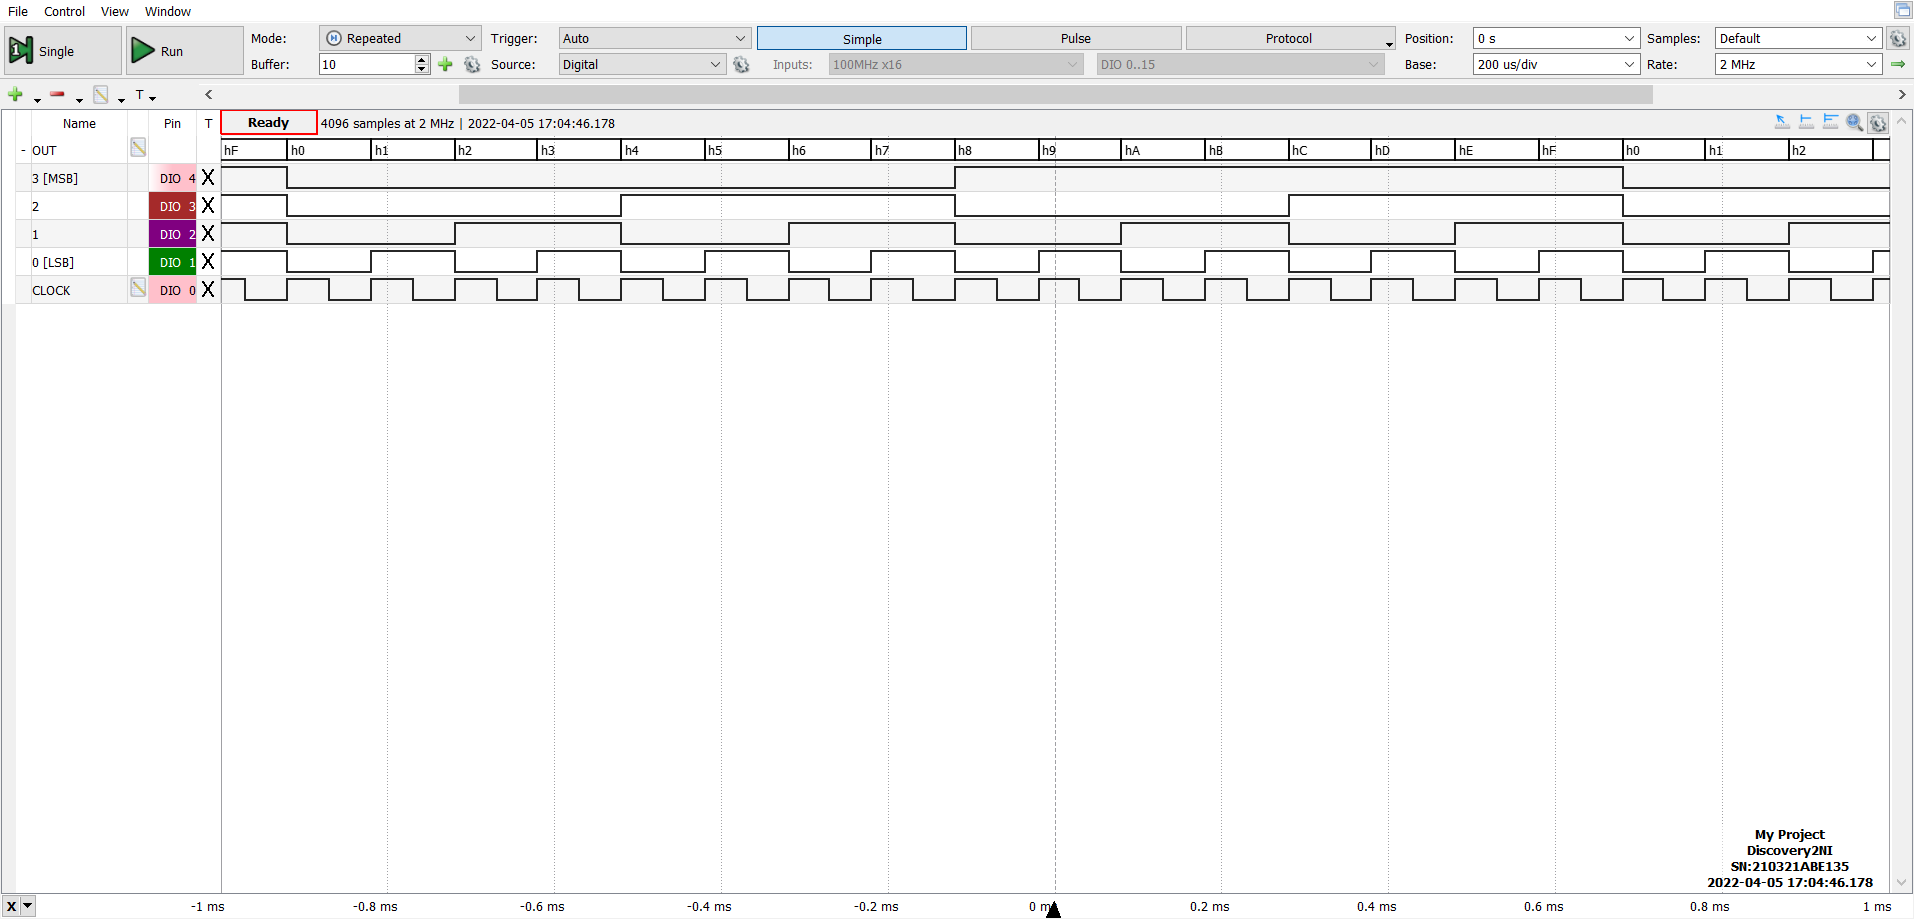
\includegraphics[width=\textwidth]{5.b}
	\label{fig: Count_Clock}
	\caption{Acquisizione temporale con Logic del bus in uscita dal contatore, con frequenza di clock pari a 10 kHz}
\end{figure}
\begin{figure}
	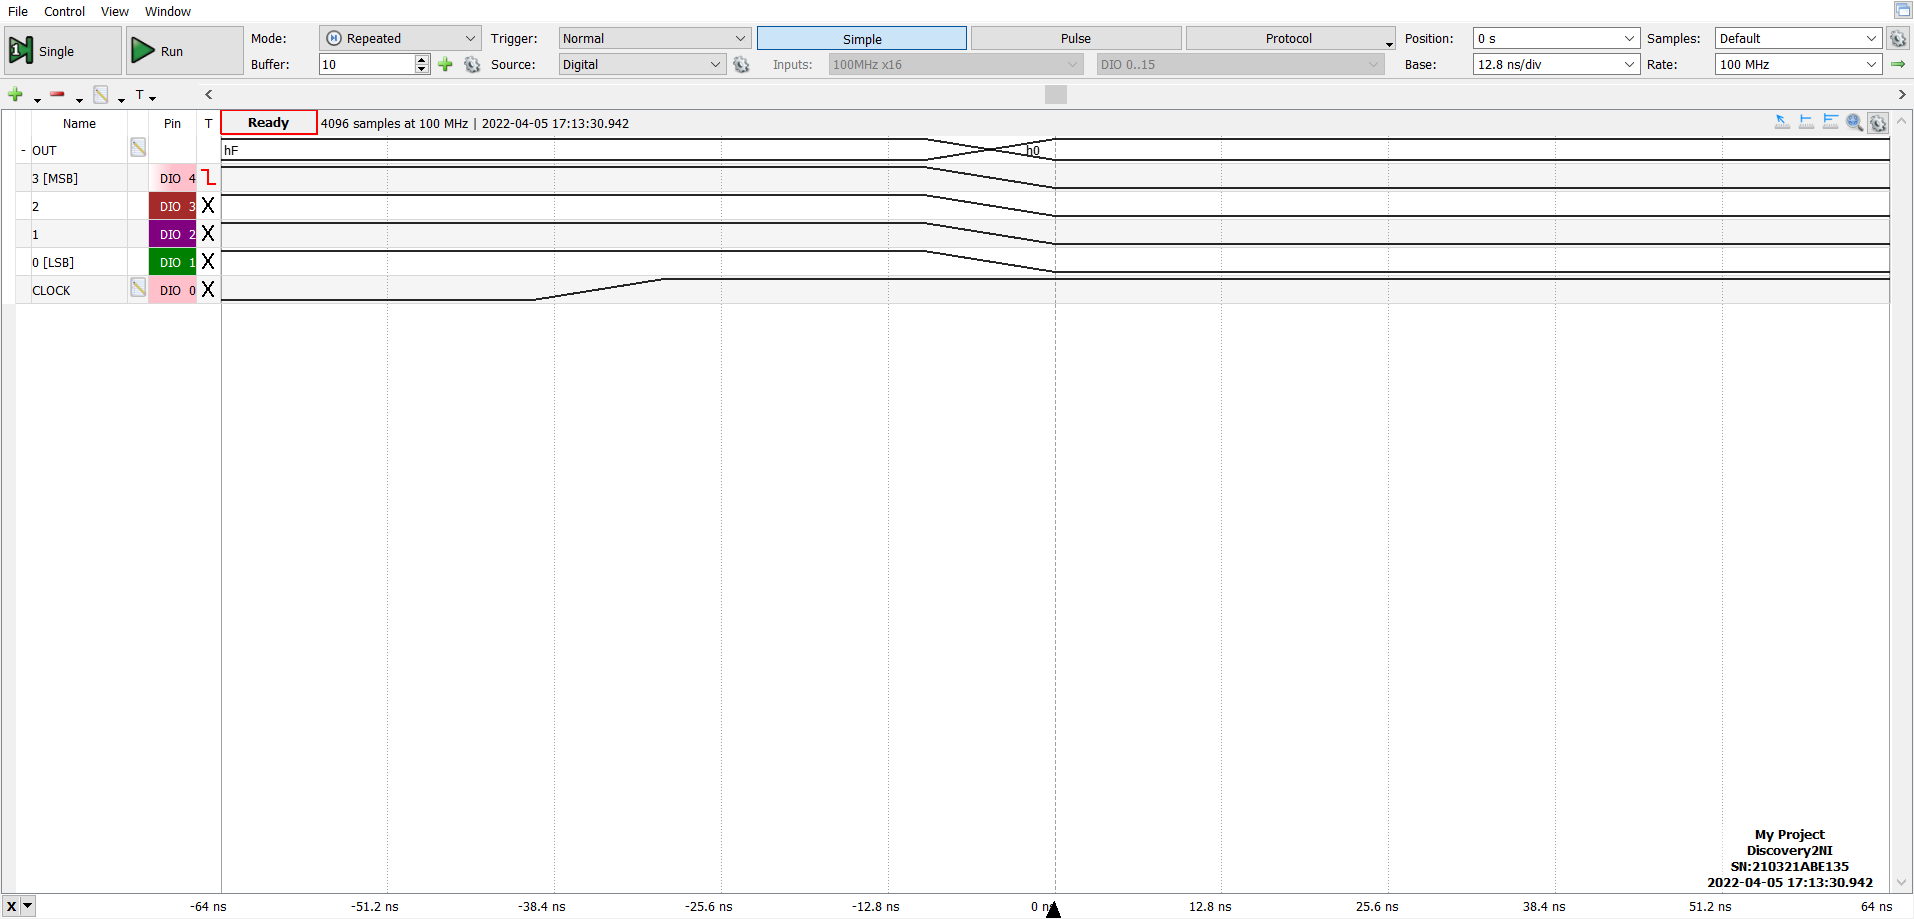
\includegraphics[width=\textwidth]{5.d}
	\label{fig: Count_150}
	\caption{Acquisizione temporale con Logic del bus in uscita dal contatore durante la transizione 15->0; dall'immagine possiamo notare il comportamento sincrono della commutazione delle uscite del contatore}
\end{figure}
\begin{figure}
	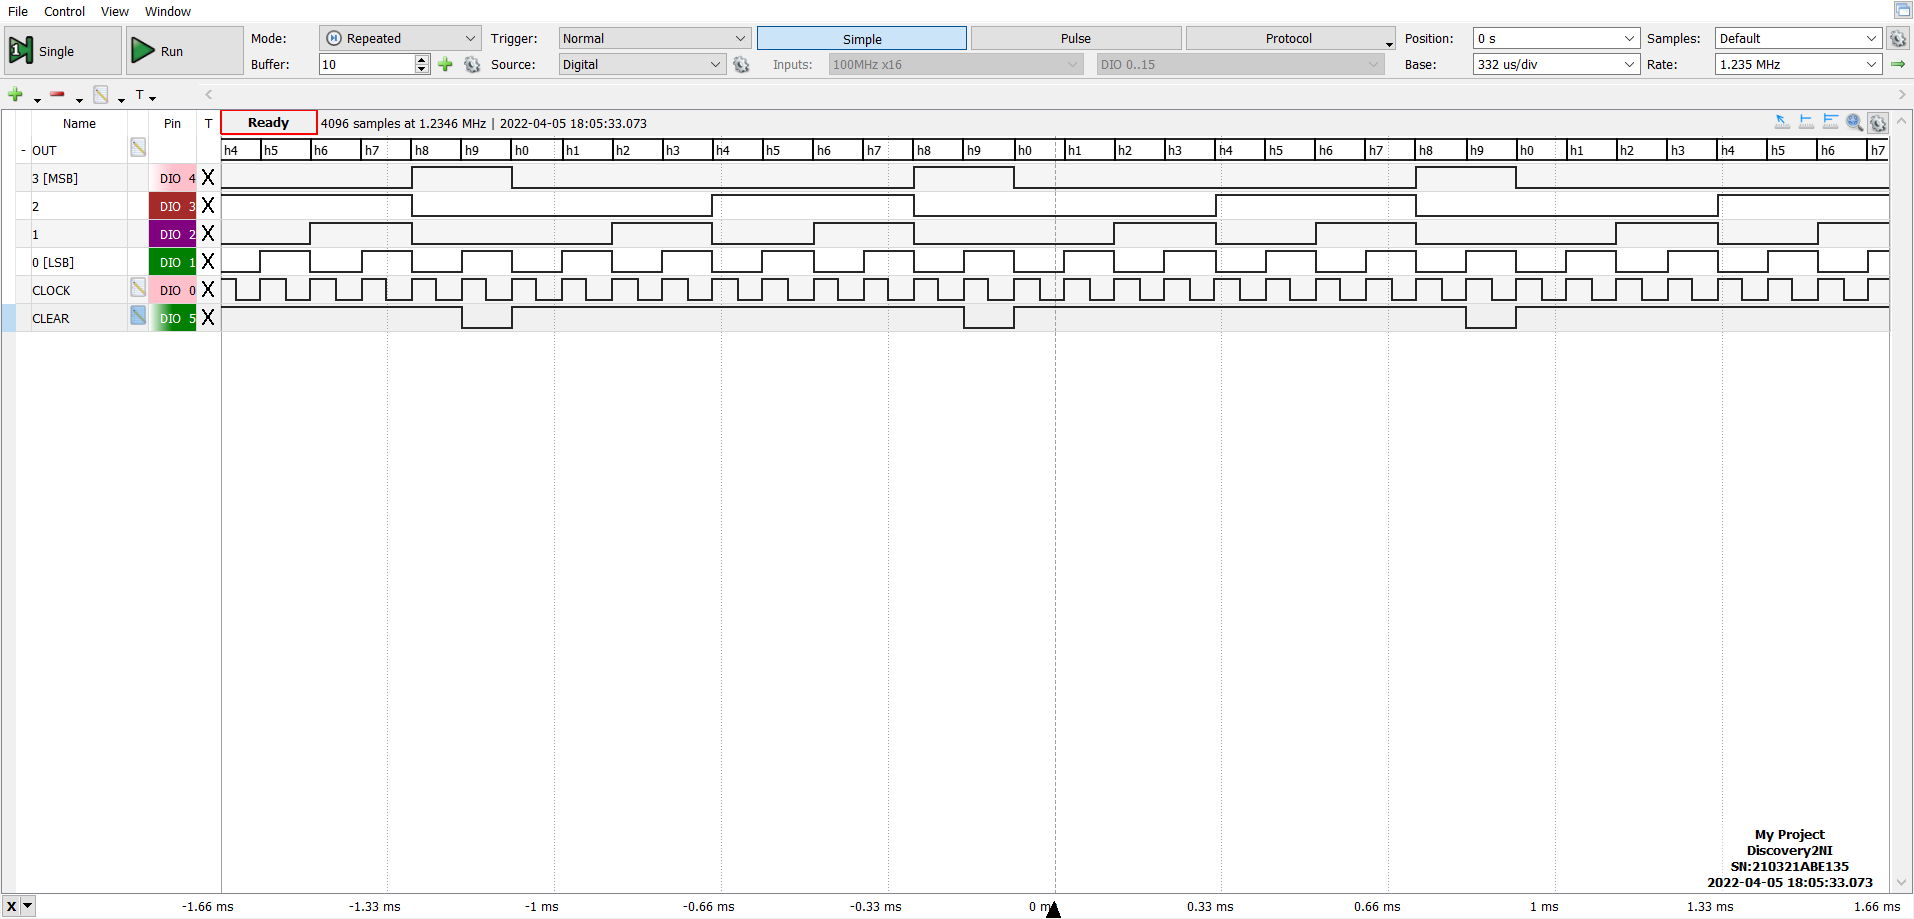
\includegraphics[width=\textwidth]{5.e}
	\label{fig: Count_10th}
	\caption{Acquisizione temporale con Logic del bus in uscita dal circuito che conta fino a 10; si può notare che il segnale in entrata nel Clock ha effettivamente periodo pari a 10 volte quello del clock}
\end{figure}
%=======================
\section*{Conclusioni e commenti finali}
Si è riusciti a verificare il corretto comportamento delle porte TTL studiate
caratterizzandone le tensioni, correnti di operazione e tempi caratteristici
di circuiti integrati come il SN7404.
Inoltre, è stato possibile verificare il funzionamento di circuiti logici di
diversa complessità costruiti con porte NAND, XOR, e OR e si è riusciti ad
apprezzare l'effetto dei tempi di propagazione delle porte nella conversione
dalla codifica Gray al binario.


%=======================
\section*{Dichiarazione}
I firmatari di questa relazione dichiarano che il contenuto della relazione \`e
originale, con misure effettuate dai membri del gruppo, e che tutti i firmatari
hanno contribuito alla elaborazione della relazione stessa.

\end{document}
